\documentclass[12pt]{article}
\usepackage[paper=letterpaper,margin=2cm]{geometry}

\usepackage{mathtools, amssymb, amsthm, amsmath}
\usepackage{enumerate}
\usepackage{enumitem}
\usepackage{fancyhdr}
\usepackage{tabularx}
\usepackage{graphicx}
\usepackage{pgfplots}
\usepackage{tikz}
\usepgfplotslibrary{polar}

\pgfplotsset{compat=newest}
\pgfplotsset{every axis/.append style={
                     tick label style={font=\footnotesize},
                 }}


\pagestyle{fancy}
\fancyhf{}
\rhead{\small {© 2022 All Rights Reserved, Aiden Rosenberg}}
\rfoot{Page \thepage}

\setlength{\droptitle}{-6em}
%\everymath{\displaystyle}

\title{AP Classroom Problems Unit 7}
\author{Aiden Rosenberg}
\date{Febuary 14, 2023 A.D}

\begin{document}
\maketitle
\section*{Notes}
\begin{align}
	\frac{dy}{dx}= \frac{\frac{dy}{d\theta}}{\frac{dx}{d\theta}} = \frac{\frac{dr}{d\theta}\sin \theta +r\cos \theta}{\frac{dr}{d\theta}\cos \theta - r\sin \theta} \\
	\frac{d^2y}{dx^2} = \frac{\frac{d}{d\theta}\big(\frac{dy}{dx}\big)}{\frac{dx}{d\theta}}                                                                         
\end{align}
\section*{7.01}
\begin{enumerate}
	\item What is the slope of the line tangent to the polar curve $r=1+2\sin \theta$ at $\theta=0$?
	      \begin{enumerate}
	      	\item $\frac{dr}{d\theta} = 2\cos \theta$
	      \end{enumerate}
	      $$\frac{dy}{dx} = \frac{2\cos\theta \cdot \sin \theta + (1+2\sin \theta) \cdot \cos\theta}{2\cos^2\theta -(1+2\sin \theta)\cdot \sin\theta}\biggr\rvert_{\theta=0} = \boxed{\frac{1}{2}}$$
	\item A polar curve is given by the equation $r=\frac{10\theta}{\theta^2+1}$ for $\theta \geq 0$. What is the instantaneous rate of change of $r$ with respect to $\theta$ when $\theta=2$?
	      $$\frac{dr}{d\theta} = \frac{-10(\theta^2-1)}{(\theta^2+1)^2}\biggr\rvert_{\theta = 2} = \boxed{\frac{-6}{5}}$$
	\item A polar curve is given by the differentiable function $r=f(\theta)$ for $0\leq \theta \leq 2\pi$. If the line tangent to the polar curve at $\theta=\frac{\pi}{3}$ is horizontal, which of the following must be true?
	      $$0=\frac{dy}{d\theta}\biggr\rvert_{\frac{\pi}{3}} = \boxed{\frac{\sqrt{3}}{2}f'\bigg(\frac{\pi}{3}\bigg)+\frac{1}{2}f\bigg(\frac{\pi}{3}\bigg)} $$
	\item For a certain polar curve $r=f(\theta)$, it is known that $\frac{dx}{d\theta} = \cos \theta - \theta\sin\theta$ and $\frac{dy}{d\theta} = \sin \theta + \theta\cos \theta$. What is the value of $\frac{d^2y}{dx^2}$ at $\theta=4$?
	      $$\frac{d^2y}{d\theta^2} = \frac{\theta^2+2}{(\cos\theta - \theta\sin\theta)^3}\biggr\rvert_{\theta = 4} \approx \boxed{1.34607}$$
	\item What is the slope of the line tangent to the polar curve $r=2\theta$ at the point $\theta=\frac{\pi}{2}$?
	      \begin{enumerate}
	      	\item $\frac{dr}{d\theta} = 2$
	      \end{enumerate}
	      $$\frac{dy}{dx} = \frac{2 \sin \theta + (2\theta) \cdot \cos\theta}{2\cos\theta -(2\theta)\cdot \sin\theta}\biggr\rvert_{\theta=\frac{\pi}{2}} = \boxed{\frac{-2}{\pi}}$$
	      	
	\item What is the slope of the line tangent to the polar curve $r = 2 \cos \theta -1$ at the point where $\theta = \pi$?
	      \begin{enumerate}
	      	\item $\frac{dr}{d\theta} = -2\sin\theta$
	      \end{enumerate}
	      $$\frac{dy}{dx} = \frac{-2\sin^2\theta + (2 \cos \theta -1)\cos\theta}{-2\sin\theta\cos\theta - (2 \cos \theta -1)\sin\theta}\biggr\rvert_{\theta = \pi} = \boxed{\frac{1}{0}}$$
	      $$\boxed{\text{Undefined}}$$ 
	\item What is the slope of the line tangent to the polar curve $r=\cos \theta$ at the point where $\theta = \frac{\pi}{6}$?
	      \begin{enumerate}
	      	\item $\frac{dr}{d\theta} = -\sin \theta$
	      	\item $\frac{dy}{d\theta} = -\sin^2\theta+\cos^2\theta $
	      	\item $\frac{dx}{d\theta}=-\sin \theta \cos \theta - \cos \theta\sin \theta$
	      \end{enumerate}
	      $$\frac{dy}{dx} = \frac{-\sin^2\theta+\cos^2\theta}{-\sin \theta \cos \theta - \cos \theta\sin \theta}\biggr\rvert_{\theta = \frac{\pi}{6}} = \boxed{\frac{-1}{\sqrt{3}}}$$
\end{enumerate}
\section*{7.02}
\begin{enumerate}
	\item 
	      \begin{center}
	      	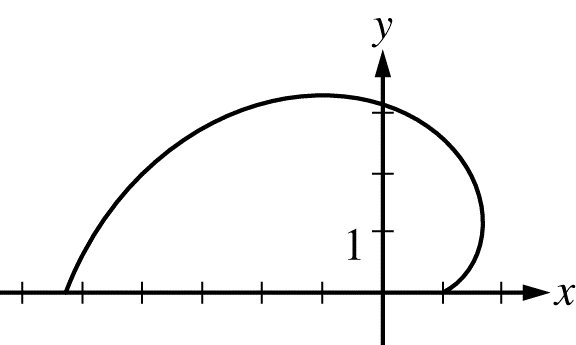
\includegraphics[width = 2in]{7.021}
	      \end{center}
	      The graph above shows the polar curve $r=2\theta + \cos\theta$ for $0\leq\theta\leq\pi$. What is the area of the region bounded by the curve and the $x$-axis?
	      $$A=\frac{1}{2} \int_{0}^{\pi} \big(2\theta + \cos\theta\big)^2\, d\theta = \frac{8\pi^3+3\pi-48}{12} \approx \boxed{17.456}$$
	\item 
	      \begin{center}
	      	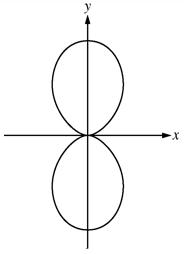
\includegraphics[width = 1.5in]{7.022}
	      \end{center}
	      Which of the following expressions gives the total area enclosed by the polar curve $r=\sin^2\theta$ shown in the figure above?
	      $$\boxed{\int_{0}^{\pi} \sin^4 \theta \, d\theta}$$
	\item 
	      \begin{center}
	      	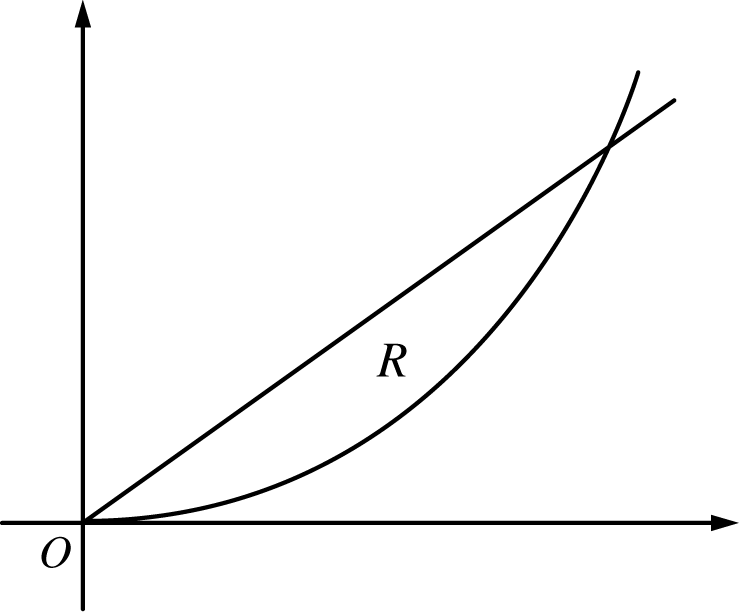
\includegraphics[width=2in]{7.023.png}
	      \end{center}
	      Let $R$ be the region in the first quadrant that is bounded by the polar curves $r=\theta$ and $\theta=k$, where $k$ is a constant, $0<k<\frac{\pi}{2}$, as shown in the figure above. What is the area of $R$ in terms of $k$?
	      $$R=\frac{1}{2}\int_{0}^{k} \theta^2 \, d\theta = \frac{\theta^3}{6}\Biggr\rvert_{0}^{k} = \boxed{\frac{k^3}{6}}$$
	\item Which of the following integrals represents the area enclosed by the smaller loop of the graph of $r=1+2\sin \theta$?
	      \begin{figure}[!h]
	      	\centering
	      	\begin{tikzpicture}[scale=0.50]
	      		\begin{polaraxis}[
	      				xtick distance = deg(pi/4),
	      				xtick = {0,0,deg((pi)/4),deg((pi)/2),deg((3*pi)/4),deg(pi),deg((5*pi)/4),deg((3*pi)/2), deg((7 * pi)/4)},
	      				xticklabels={0,0,$\frac{\pi}{4}$,$\frac{\pi}{2}$,$\frac{3\pi}{4}$,$\pi$,$\frac{5\pi}{4}$,$\frac{3\pi}2$, $\frac{7\pi}{6}$ }
	      			]
	      			\addplot[domain=0:2*pi,samples=100,color=red,data cs=polarrad] { 1 + 2*sin(deg(x)) };
					  \addlegendentry{$r=1+2\sin \theta$}
	      		\end{polaraxis}
	      			   
	      	\end{tikzpicture}
	      \end{figure}
	      
	      \begin{enumerate}
	      	\item $0 =1+2\sin \theta$ when $\theta = \frac{7\pi}{6}$ and $\theta = \frac{11\pi}{6}$
	      \end{enumerate}
	      $$\boxed{A=\frac{1}{2}\int_{\frac{7\pi}{6}}^{\frac{11\pi}{6}}\big(1+2\sin \theta\big)^2 \, d\theta}$$
		  \pagebreak
	\item Which of the following gives the total area enclosed by the graph of the polar curve $r = \theta \sin 2\theta$ for $0\leq\theta\leq 2\pi$?

	\begin{figure}[!h]
		\centering
		\begin{tikzpicture}[scale=0.50]
			\begin{polaraxis}[
					xtick distance = deg(pi/4),
					xtick = {0,0,deg((pi)/4),deg((pi)/2),deg((3*pi)/4),deg(pi),deg((5*pi)/4),deg((3*pi)/2), deg((7 * pi)/4)},
					xticklabels={0,0,$\frac{\pi}{4}$,$\frac{\pi}{2}$,$\frac{3\pi}{4}$,$\pi$,$\frac{5\pi}{4}$,$\frac{3\pi}2$, $\frac{7\pi}{6}$ }
				]
				\addplot[domain=0:2*pi,samples=100,color=red,data cs=polarrad] { x*sin(2* deg(x)) };
				\addlegendentry{$r=\theta \sin 2\theta$}
			\end{polaraxis}
		\end{tikzpicture}
	\end{figure}
	$$A = \boxed{\frac{1}{2} \int_{0}^{2\pi} |\theta\sin2\theta|^2 \, d\theta}$$
	\item Which of the following integrals gives the area of the region that is bounded by the graphs of the polar equations $\theta=0$, $\theta = \frac{\pi}{4}$, and, $r=\frac{2}{\cos \theta+\sin\theta}$? 

	\begin{figure}[!h]
		\centering
		\begin{tikzpicture}[scale=0.50]
			\begin{polaraxis}[
					ymax= 2,
					xtick distance = deg(pi/4),
					xtick = {0,0,deg((pi)/4),deg((pi)/2),deg((3*pi)/4),deg(pi),deg((5*pi)/4),deg((3*pi)/2), deg((7 * pi)/4)},
					xticklabels={0,0,$\frac{\pi}{4}$,$\frac{\pi}{2}$,$\frac{3\pi}{4}$,$\pi$,$\frac{5\pi}{4}$,$\frac{3\pi}2$, $\frac{7\pi}{6}$ }
				]
				\addplot[domain=0:2*pi,samples=100,color=red,data cs=polarrad] { 2*(sin(deg(x)) + cos(deg(x)))^(-1)};  
				\addlegendentry{$r=\frac{2}{\cos \theta+\sin\theta}$}

			\end{polaraxis}
				   
		\end{tikzpicture}
	\end{figure}
	$$A= \boxed{\int_{0}^{\frac{\pi}{4}} \frac{2}{\big(\cos \theta +\sin\theta\big)^2} \, d\theta}$$
\end{enumerate}
\section*{7.03}
\begin{enumerate}
	\item What is the total area between the polar curves $r = 5 \sin(3\theta)$ and $r = 8 \sin(3\theta)$?
	$$A = \frac{1}{2} \int_{0}^{\pi} \bigg(\big(8\sin(3\theta))^2 - \big(5\sin(3\theta\big)^2\bigg)\, d\theta \approx \boxed{30.631}$$
	\item 
	      \begin{center}
	      	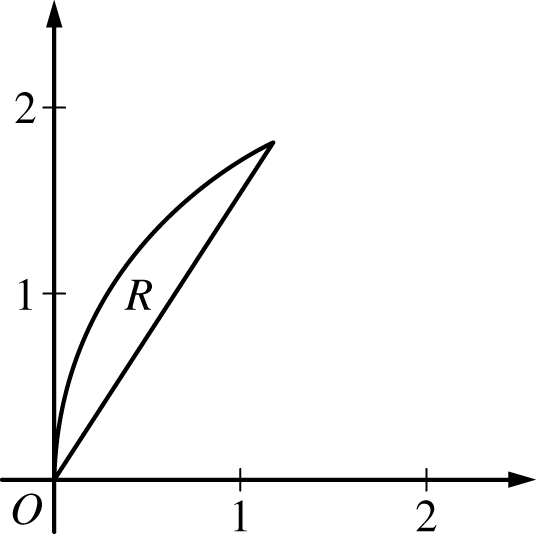
\includegraphics[width=2in]{7.032.png}
	      \end{center}
	      Let $R$ be the region in the first quadrant that is bounded above by the polar curve $r=4\cos \theta$ and below by the line $\theta=1$, as shown in the figure above. What is the area of $R$?
	$$R = \frac{1}{2}\int_{1}^{\frac{\pi}{2}}\big(4\cos\theta\big)^2\, d\theta =-2(\sin(2)-\pi+2) \approx \boxed{0.465}$$
	\item 
	      \begin{center}
	      	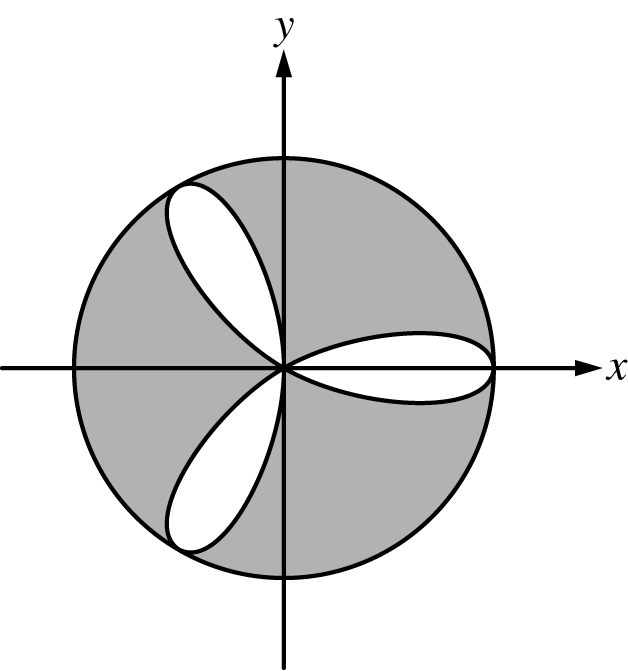
\includegraphics[width = 2in]{7.033.png}
	      \end{center}
	      The figure above shows the graphs of the polar curves $r=2\cos(3\theta)$and $r=2$. What is the sum of the areas of the shaded regions?
	$$A=\underbrace{4\pi}_{\text{Area of circle}} - \underbrace{\frac{1}{2}\int_{0}^{\pi} (2\cos(3\theta))^2}_{\text{Area of rose}} = 3\pi \approx \boxed{9.425}$$
	\item What is the area of the region $R$ bounded by the graph of the polar curve $r=\sqrt{1+\frac{3\theta}{\pi}}$ and the $x$-axis for $0\leq\theta\leq\pi$?
	$$R = \frac{1}{2} \int_{0}^{\pi} \bigg(1+\frac{3\theta}{\pi}\bigg) \, d\theta = \frac{1}{2} \bigg[\theta + \frac{3\theta^2}{2\pi}\bigg]_{0}^{\pi} = \boxed{\frac{5\pi}{4}}$$
	\item 
	      \begin{center}
	      	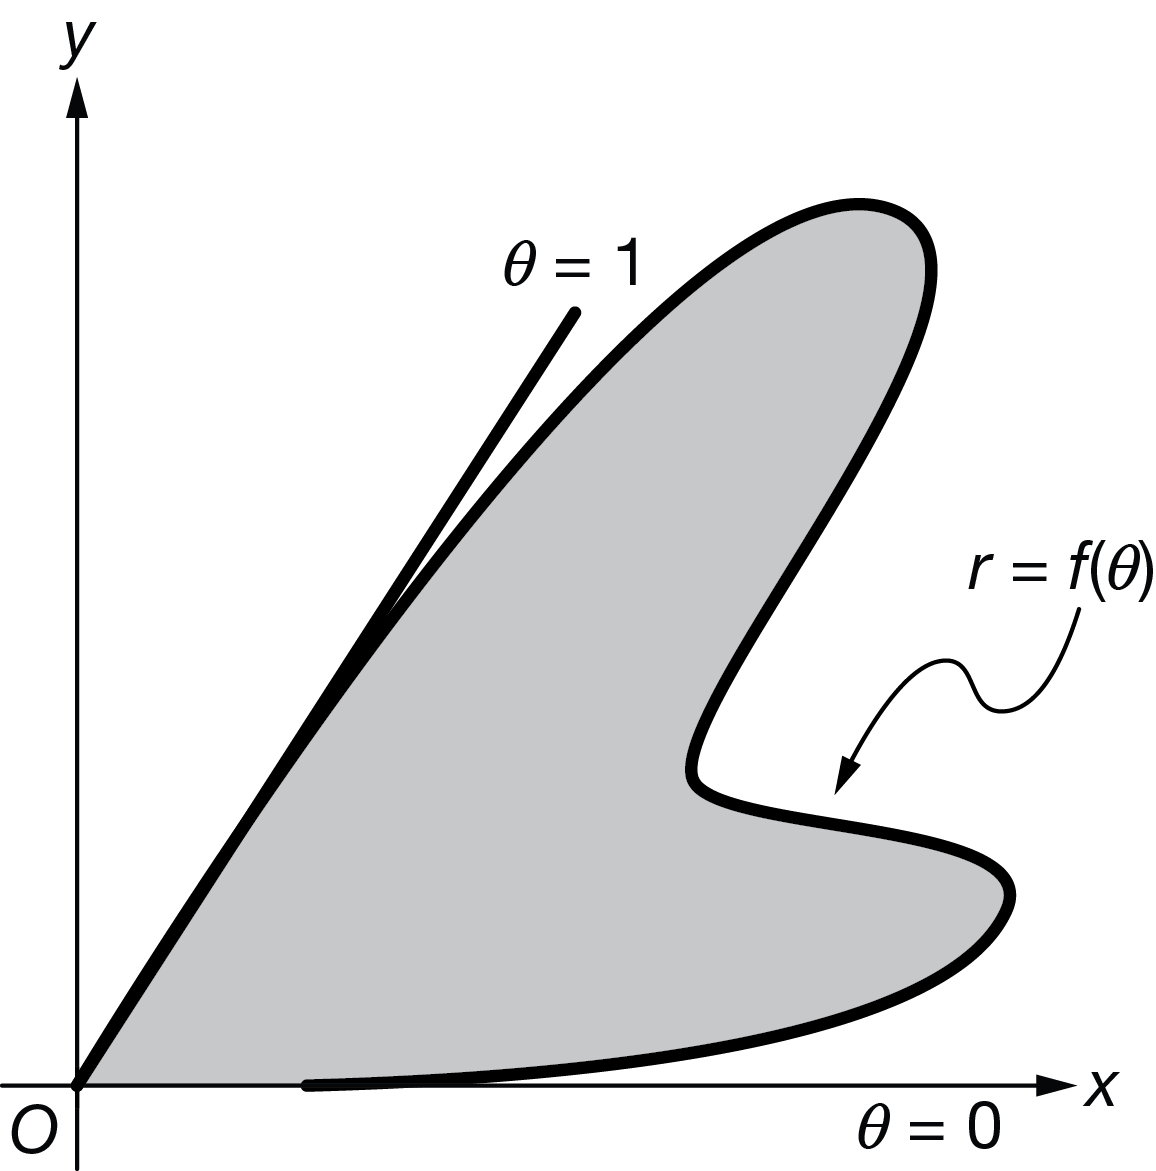
\includegraphics[width = 2in]{7.035}
	      \end{center}
	      \begin{table}[h]
	      	\centering
	      	\begin{tabular}{c|c|c|c|c|c}
	      		$\theta$ & $0$ & $\frac{1}{4}$ & $\frac{1}{2}$ & $\frac{3}{4}$ & $1$ \\ \hline
	      		$r$      & $1$ & $4$           & $3$           & $5$           & $2$ 
	      	\end{tabular}
	      \end{table}
	      Let $R$ be the region bounded by the graph of the polar curve $r=f(\theta)$ and the lines $\theta=0$ and $\theta=1$, as shaded in the figure above. The table above gives values of the polar function $r=f(\theta)$ at selected values of $\theta$. What is the approximation for the area of region $R$ using a right Riemann sum with the four subintervals indicated by the data in the table?
		  \begin{enumerate}
			\item Note that Area $\approx \sum_{i=1}^{n} \frac{1}{2} r(\theta_i)^2 \, \Delta \theta$
		  \end{enumerate}
		  $$A = \frac{1}{2}\cdot \underbrace{\frac{1}{4}}_{\Delta\theta \cdot}\biggr(f\Big(\frac{1}{4}\Big)^2+f\Big(\frac{1}{2}\Big)^2 + f\Big(\frac{3}{4}\Big)^2\biggr) \approx \boxed{\frac{1}{8}(16+9+25+4)}$$
	\item 
	      \begin{center}
	      	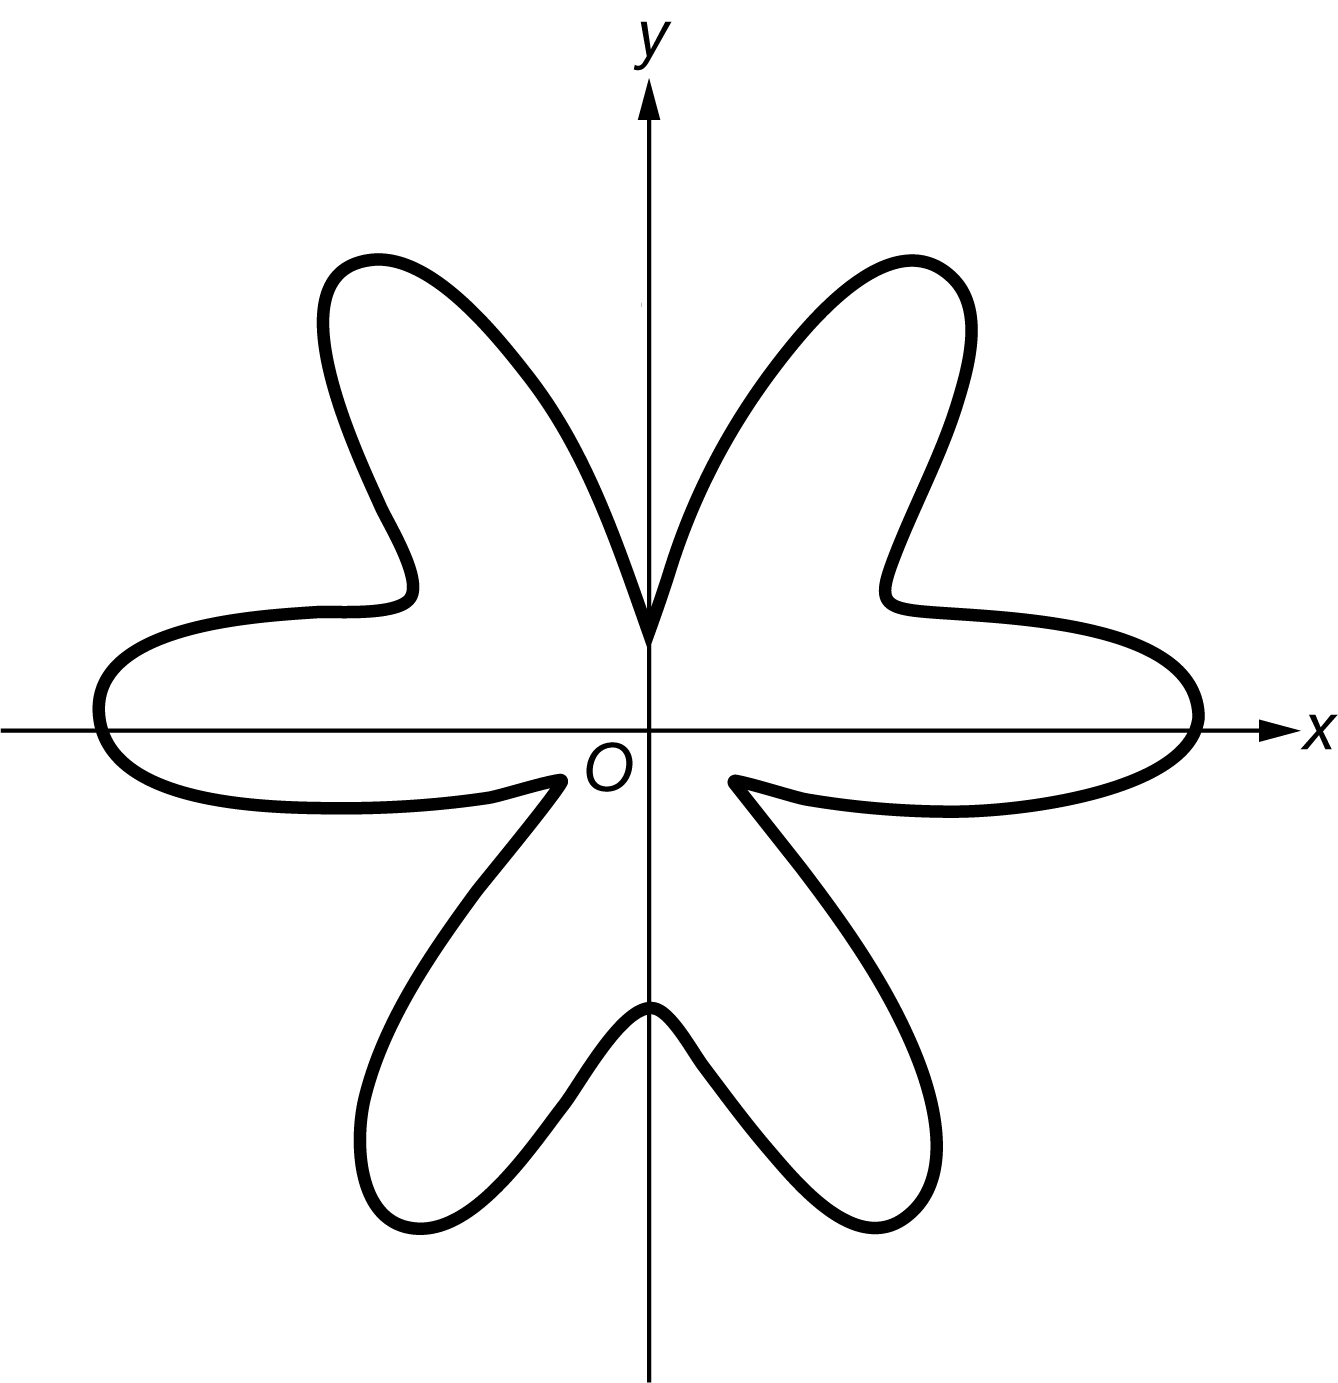
\includegraphics[width = 2in]{7.036}
	      \end{center}
	      What is the area of the region bounded by the graph of the polar curve $r= 1 + \frac{1}{2}\cos(6\theta) + \frac{1}{4} \sin(3\theta)$, shown in the figure above?
		  $$A=\frac{1}{2} \cdot\int_{0}^{2\pi} \bigg(1 + \frac{1}{2}\cos(6\theta) + \frac{1}{4} \sin(3\theta)\bigg) \, d\theta = \frac{37\pi}{32} \approx \boxed{3.632}$$
	\item 
	      \begin{center}
	      	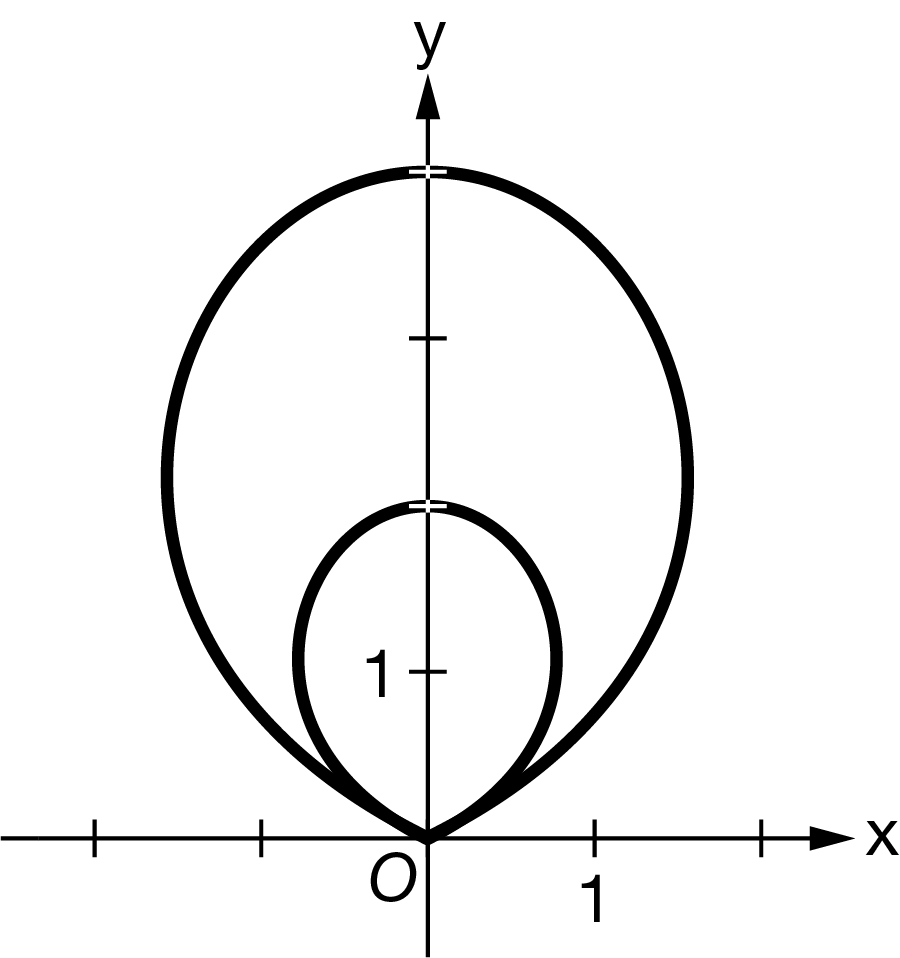
\includegraphics[width=2in]{7.037}
	      \end{center}      
	      The figure above shows the graphs of the polar curves $r=2\sin^2\theta$ and $r=4\sin^2\theta$ for $0\leq \theta\leq\pi$. Which of the following integrals gives the area of the region bounded between the two polar curves?
		  $$A = \frac{1}{2} \int_{0}^{\pi} \bigg(\big(4\sin^2\theta\big)^2 - \big(2\sin^2\theta\big)\bigg)\, d\theta  = \boxed{\int_{0}^{\pi} 6\sin^2\theta \, d\theta}$$
\end{enumerate}
\end{document}